%%% LaTeX Template: Two column article
%%%
%%% Source: http://www.howtotex.com/
%%% Feel free to distribute this template, but please keep to referal to http://www.howtotex.com/ here.
%%% Date: February 2011

%%% Preamble
\documentclass[    DIV=calc, paper=a4,fontsize=11pt, twocolumn]{scrartcl}                     % KOMA-article class

\usepackage{lipsum}                                                    % Package to create dummy text
\usepackage[utf8]{inputenc}
\usepackage{listings}
\usepackage[croatian]{babel}
\usepackage[protrusion=true,expansion=true]{microtype}                % Better typography
\usepackage{amsmath,amsfonts,amsthm}                                % Math packages
\usepackage[pdftex]{graphicx}                                        % Enable pdflatex
\usepackage[svgnames]{xcolor}                                        % Enabling colors by their 'svgnames'
\usepackage[hang, small,labelfont=bf,up,textfont=it,up]{caption}    % Custom captions under/above floats
\usepackage{epstopdf}                                                % Converts .eps to .pdf
\usepackage{subfig}                                                    % Subfigures
\usepackage{booktabs}                                                % Nicer tables
\usepackage{fix-cm}                                                    % Custom fontsizes

\usepackage{algorithmic}


%%% Custom sectioning (sectsty package)
\usepackage{sectsty}                                                % Custom sectioning (see below)
\allsectionsfont{%                                                    % Change font of al section commands
    \usefont{OT1}{phv}{b}{n}%                                        % bch-b-n: CharterBT-Bold font
    }

\sectionfont{%                                                        % Change font of \section command
    \usefont{OT1}{phv}{b}{n}%                                        % bch-b-n: CharterBT-Bold font
    }



%%% Headers and footers
\usepackage{fancyhdr}                                                % Needed to define custom headers/footers
    \pagestyle{fancy}                                                % Enabling the custom headers/footers
\usepackage{lastpage}    

% Header (empty)
\lhead{}
\chead{}
\rhead{}
% Footer (you may change this to your own needs)
\lfoot{\footnotesize Q Learning}
\cfoot{}
\rfoot{\footnotesize page \thepage\ of \pageref{LastPage}}            % "Page 1 of 2"
\renewcommand{\headrulewidth}{0.0pt}
\renewcommand{\footrulewidth}{0.4pt}



%%% Creating an initial of the very first character of the content
\usepackage{lettrine}
\newcommand{\initial}[1]{%
     \lettrine[lines=3,lhang=0.3,nindent=0em]{
                     \color{DarkGoldenrod}
                     {\textsf{#1}}}{}}



%%% Title, author and date metadata
\usepackage{titling}                                                % For custom titles

\newcommand{\HorRule}{\color{DarkGoldenrod}%                        % Creating a horizontal rule
                                          \rule{\linewidth}{1pt} }
\pretitle{\vspace{-30pt} \begin{flushleft} \HorRule
                \fontsize{50}{50} \usefont{OT1}{phv}{b}{n} \color{DarkRed} \selectfont
                }
\title{Q Learning}                                                    % Title of your article goes here
\posttitle{\par\end{flushleft}\vskip 0.5em}

\preauthor{\begin{flushleft}
                    \large \lineskip 0.5em \usefont{OT1}{phv}{b}{sl} \color{DarkRed}}
\author{Ivan Androš, Dejan Peretin, Petra Podolski, }                % Author name goes here
\postauthor{\footnotesize \usefont{OT1}{phv}{m}{sl} \color{Black}
                    PMF - Matematički odsjek, Zagreb                 % Institution of author
                    \par\end{flushleft}\HorRule}

\date{Svibanj 2011.}                                                


%%% Begin document
\begin{document}
\maketitle
\thispagestyle{fancy}                                                 % Enabling the custom headers/footers for the first page
% The first character should be within \initial{}
\initial{Q}Learning je jedna od tehnika učenja s podrškom. Agent uči iz svog iskustva bez učitelja, tako da ispituje stanje po stanje sve dok ne dođe do cilja. Svaki takav ciklus istraživanja jednog stanja naziva se epizoda. Konkretno, agent uči evaluacijsku funkciju $Q:S\times A\to \mathbb{R}$ gdje je $S$ skup stanja, a $A$ skup akcija. Poduzimajući akcije, agent se kreće iz stanja u stanje, a za svako stanje "dobiva" nagradu (realni broj) koji pokazuje korisnost stanja. Cilj agenta je maksimizirati nagradu. Konvergencija ovog algoritma se može dokazati. Agentu ne mora biti poznat model okoliša, jer bi se u tom slučaju mogao iskoristiti neki od bržih algoritama.

\section*{Opis algoritma Q learning i primjer}
Zamislimo da imamo robota kojeg moramo naučiti kako da se kreće po nekom prostoru npr. stanu koji se sastoji od nekoliko soba i vrata koja ih povezuju. Ako se s početne točke počne kretati u proizvoljnom smjeru, velika je vjerojatnost da će do\'{c}i do zida i neće moći dalje. To se može smatrati nepoželjnijim stanjem nego prolazak kroz vrata u drugu sobu. Učenje bi se u tom slučaju odvijalo tako da se za svaki sudar sa zidom daje minimalna nagrada, a za prolazak kroz vrata veća, a za stizanje na cilj najveća nagrada. Pogledajmo ipak jednostavniji primjer na slici \ref{fig:1}; prikazan je tlocrt stana koji se sastoji od 5 soba i 6 vrata, a zadatak agenta je izaći van.

\begin{figure}
\centering
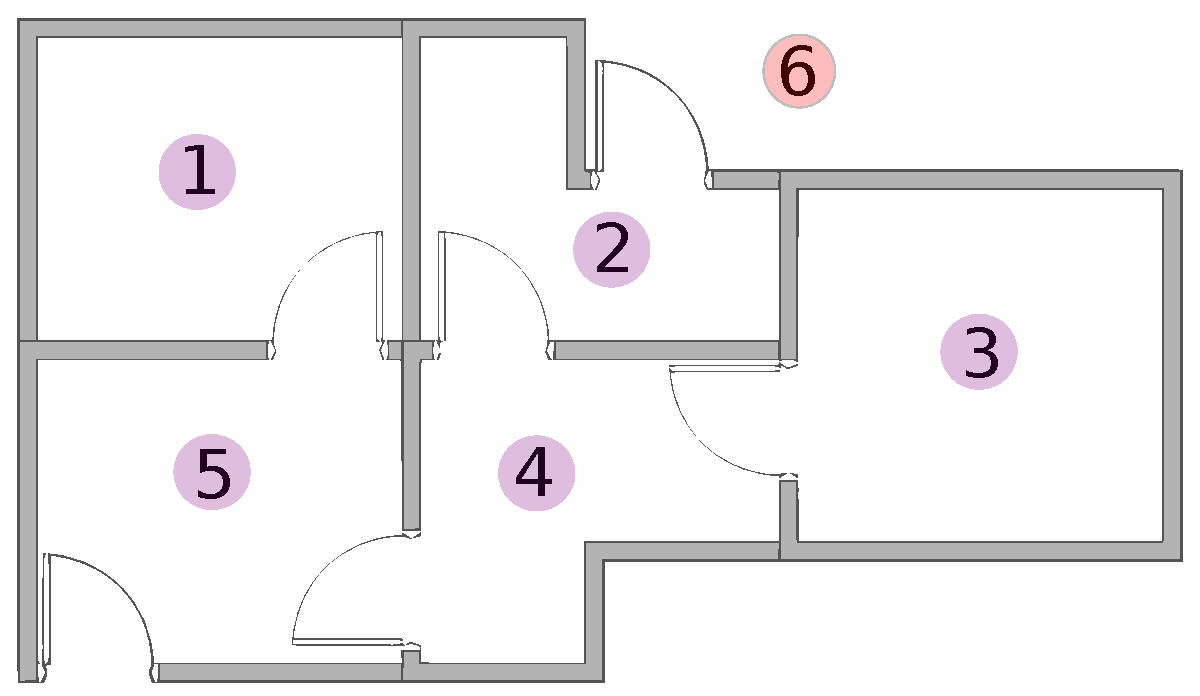
\includegraphics[scale=0.4]{slike/soba.pdf}
\caption{Agent se nalazi u jednoj od soba, mora izaći van}
\label{fig:1}
\end{figure}

Isti problem je prikazan dijagramom na slici \ref{fig:2}.
Stanja su prikazana krugovima, a akcije koje agenta vode iz stanja u stanje strelicama s težinama. Inicijalno su sve težine postavljene na $0$, osim za one akcije koje agenta vode u ciljno stanje, one imaju težinu jednaku 100.

\begin{figure}[h!]
\centering
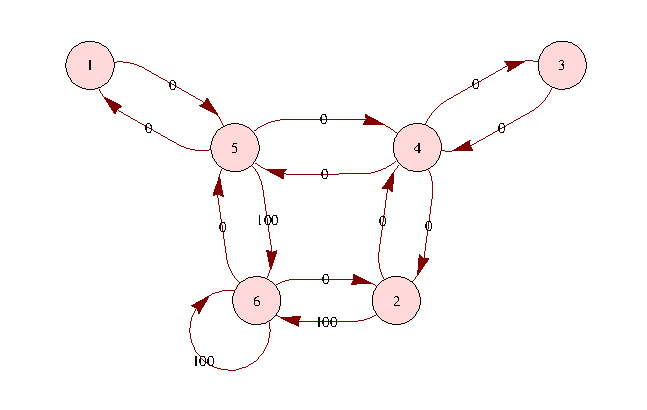
\includegraphics[scale=0.8]{slike/R.pdf}
\caption{Dijagram stanja prethodnog tlocrta}
\label{fig:2}
\end{figure}

U algoritmu se koriste dvije $n \times n$ matrice; matricu okoliša $R$ i matricu učenja $Q$. Matrica $R$ predstavlja dijagram stanja. Ako su stanja $i$ i $j$ susjedna (povezana), u matrici će na mjestu $(i, j)$ pisati $0$ (ili u modificiranoj verziji programa, težina $\omega \in \mathbb{R}$), ako se iz stanja $i$ prelazi u stanje $j$ koje je ciljno, u matrici na mjestu $(i, j)$ pisat će $100$, a ako dva stanja nisu susjedna, vrijednost u matrici bit će $-\inf$. Matrica $Q$ na početku sadrži $0$ na svim mjestima.


\subsection*{Pseudokod učenja funkcije Q}
\begin{algorithmic}
\STATE učitaj parametar $\gamma$ i matricu $R$
\STATE inicijaliziraj vrijednosti matrice $Q$ na 0
\WHILE{nema konvergencije}
\STATE na slučajan način izaberi inicijalno stanje
\WHILE{nismo u završnom stanju}
\STATE izaberi jedno od mogućih akcija za trenutno stanje
\STATE $Q_{s, a} = R_{s, a}+\gamma \cdot \max_i\{Q_{a, a_i}\}$
\STATE postavi sljedeće stanje za trenutno stanje
\ENDWHILE
\ENDWHILE
\end{algorithmic}

Pomoću ovog algoritma agent uči iz svog iskustva tj. treninga. U svakoj epizodi agent istražuje svoj okoliš (matrica $R$) i (ne) dobiva nagradu ako (ne) dođe do cilja. Što dulje uči (tj. što više epizoda izvede), bolje će upoznati svoj okoliš i više naučiti (tj. naći će točniju matricu $Q$).
Parametar $\gamma$ je unaprijed izabrana vrijednost između $0$ i $1$. Više o značenju parametra $\gamma$ kasnije je objašnjeno uz sliku \ref{fig:5}.

Kad je $Q$ matrica završena, iz nje je lako pročitati slijed akcija koji daje najbrži put od nekog početnog do ciljnog stanja.

\subsection*{Pseudokod nalaženja najkraćeg puta}
\begin{algorithmic}
\STATE učitaj matricu $Q$ i početno stanje
\WHILE{trenutno stanje != finalno stanje}
\STATE za trenutno stanje nađi akciju koja ima najveću vrijednost u matrici $Q$
\STATE za trenutno stanje odaberi ono stanje u koje vodi prethodno odabrana akcija
\ENDWHILE
\end{algorithmic}

\begin{figure}[h!]
\centering
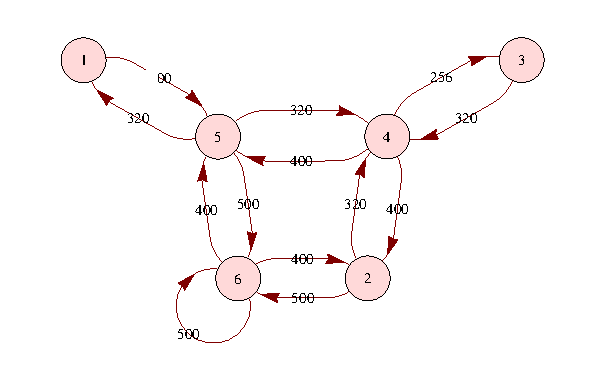
\includegraphics[scale=0.9]{slike/Q.pdf}
\caption{Dijagram stanja iz perspektive funkcije $Q$}
\end{figure}


\section*{Implementacija}
Q learning smo implementirali u programskom jeziku python. Zašto python? Jezik python stvoren je s ciljem lake čitljivosti, velike snage s jednostavnom sintaksa, što omogućuje brzo prototipiranje.
Cilj ovog projekta nije bio napraviti jako brzi program, nego ispitati skalabilnost algoritma. Dodatne prednosti pythona su mogućnost integracije sa matematičkim softverom SAGE te vrlo dobro skaliranje sa sve boljim poznavanjem problema.

\subsection*{Generiranje grafova}
Kreiranje algoritam za slučajno generiranje problema - grafova je jednako (ako ne i više) težak problem od samog Q learning algoritma. To što komplicira problem su uvjeti koje traženi graf mora zadovoljavati:
\begin{itemize}
\item
Mora biti povezan.
\item
Ne smije biti \emph{pregust}.
\item
Na slučajan način generiramo nagrade.
\end{itemize}

Da bismo mogli bolje analizirati dobivene rezultate, stvorili smo dvije vrste grafova, nazvali smo ih \emph{gusti} i \emph{dugi}.

U gustim grafovima čvorovi su povezani s relativno malo drugih čvorova. Većina veza je između čvorova koji su \emph{blizu} te
čvor može biti povezan s najviše jednim čvorom koji mu nije blizu.

U dugim grafovima čvorovi su povezani s nekoliko \emph{najbližih} čvorova, dakle sve veze su između čvorova koji su \emph{blizu}.


\section*{Korištenje programa}
Program se sastoji od sljedećih funkcija:

\vspace{0.4cm}
\noindent\textbf{\texttt{Generate(size, cilj, tip='gusta', raspon=(0, 0))}}
\begin{itemize}
\item    $size$  - broj stanja u dijagramu
\item    $cilj$  - index ciljnog čvora, brojeći od 0. Nagrada je automatski postavljena na 100.
\item    $tip$   - tip matrice koja se generira.
Default vrijednost je 'gusta' - stanja mogu biti povezana sa svim stanjima, ali je mala vjerojatnost da bude povezana sa stanjima koja su daleko. Druga mogućnost je 'duga' - stanja mogu biti povezana samo sa nekoliko najbli\v{z}ih stanja
\item    $raspon$ - uređen par cijelih brojeva $(a, b)$, vrijednosti matrice $a$ su iz segmenta $[a, b]$
\end{itemize}
Funkcija vraća matricu nagrada sljedećeg formata:
\begin{itemize}
\item         - ako stanja $x$ i $y$ nisu spojena, $m(x, y) = -inf$
\item         - ako jesu spojena, $m(x, y) = z \in [a, b]$
\end{itemize}

\vspace{0.4cm}
\noindent\textbf{\texttt{ToString(matrica)}}

   Sprema matricu u jedan string, redovi su odvojeni znakom '\textbackslash n', 
   a elementi reda zarezom.
   
\vspace{0.4cm}
\noindent\textbf{\texttt{AdjacencyMatrix(matrica)}}

    Iz matrice generira matricu susjedstva koja se može koristiti za crtanje grafova softverom kao što je SAGE ili Mathematica.

\vspace{0.4cm}
\noindent\textbf{\texttt{Parse(cijeliFajl)}}

    Iz stringa koji sadrži informacije o dijagramu stanja, koji je spremljen kao niz vrijednosti odvojenih zarezom, a redovi su odvojeni znakom '\textbackslash n', 
    generira se matrica koja se može koristiti za učenje.

\vspace{0.4cm}
\noindent\textbf{\texttt{Imp(x, n=7)}}

    Improved Matrix Print - Ispisuje matricu u oku ugodnom formatu.

\vspace{0.4cm}
\noindent\textbf{\texttt{LearnQ(R, gamma, kraj, bench=False)}}

    Vraća matricu $Q$. Pri tomu je:
\begin{itemize}
\item    $R$     - matrica nagrada,
\item    $gamma$ - koeficijent,
\item    $kraj$  - ciljni čvor, brojeći od 0,
\item    $bench$ - False (default) ili True - uz matricu $Q$ vraća i broj izvršenih epizoda i broj koraka algoritma kao uređenu trojku
\end{itemize}

\vspace{0.4cm}
\noindent\textbf{\texttt{FindPath(Q, poc, kraj)}}

    Vraća listu čvorova koji tvore najkraći put od čvora $poc$ do čvora $kraj$, prema matrici $Q$.
    
\vspace{0.4cm}
Budući da je program napisan u pythonu, jedini preduvjet za njegovo izvršavanje je instaliran python na računalu.
Nadalje, program nije kompiliran u strojni kod nego se prilikom pokretanja interpretira, pa program mora biti
svjestan putanje to python interpretera. Pretpostavljena lokacija je \texttt{/usr/bin/python}, ukoliko to nije slučaj na
računalu na kojem se želi pokrenuti program, putanju treba podesiti u prvoj liniji programa ili program pokrenuti direktno iz
pythona.

Sam program se može koristiti na dva načina. Prvi način je direktno pokretanje na danom problemu.
Ako primjerice imamo u datoteci \texttt{R.mat} zapisanu matricu $R$ i zanima nas najkraći put od čvora 0 do ciljnog čvora 5, 
to možemo dobiti sa:

\begin{center}
\texttt{qlearning.py R.mat 0 5}
\end{center}
ili:
\begin{center}
\texttt{python qlearning.py R.mat 0 5}
\end{center}
Put se ispisuje na standardni izlaz. Npr:
\begin{center}
\texttt{0 -> 4 -> 5}
\end{center}

Drugi način korištenja programa je kao \emph{modul}, tj. korisnik može sam napisati program koristeći funkcije 
koje su definirane u programu. Primjer programa koji oponaša defaultni rad našeg programa bi bio:

\lstset{ %
language=Python,                % the language of the code
basicstyle=\footnotesize,       % the size of the fonts that are used for the code
                   % the step between two line-numbers. If it's 1, each line 
                                % will be numbered
numbersep=5pt,                  % how far the line-numbers are from the code
backgroundcolor=\color{white},  % choose the background color. You must add \usepackage{color}
showspaces=false,               % show spaces adding particular underscores
showstringspaces=false,         % underline spaces within strings
showtabs=false,                 % show tabs within strings adding particular underscores
frame=none,                   % adds a frame around the code
tabsize=2,                      % sets default tabsize to 2 spaces
captionpos=b,                   % sets the caption-position to bottom
breaklines=true,                % sets automatic line breaking
breakatwhitespace=false,        % sets if automatic breaks should only happen at whitespace
title=\lstname,                 % show the filename of files included with \lstinputlisting;
                                % also try caption instead of title
escapeinside={\%*}{*)},         % if you want to add a comment within your code
morekeywords={*,...}            % if you want to add more keywords to the set
}

\begin{lstlisting}
import sys
import qlearning as QL
filename = sys.argv[1]
poc = int(sys.argv[2])
kraj = int(sys.argv[3]) 
f = open(filename, 'rU')
cijeliFajl = f.read()
R = QL.Parse(cijeliFajl)
Q = QL.LearnQ(R, 0.8, kraj)
P = QL.FindPath(Q, poc, kraj)    
print ' -> '.join(map(str, P))
\end{lstlisting}

\section*{Rezultati i zaključak}
Na slici \ref{fig:3} vidimo odnos broja koraka algoritma s obzirom na broj stanja. Taj odnos je očekivano približno linearan. Mjerenja su izvršena tako da se za svaki fiksirani broj stanja generiralo 10 grafova i onda se uzela aritmetička sredina broja koraka od tih 10 slučajeva. Ovdje treba napomenuti da ti brojevi dosta variraju jer se počeci epizoda algoritma biraju na slučajan način, pa se obzirom na odabir, algoritam može završiti i puno brže, ali i puno sporije. To je također razlog zašto ne možemo analizom algoritma (brojanjem koraka) odrediti njegovu složenost.

\begin{figure}[h!]
\centering
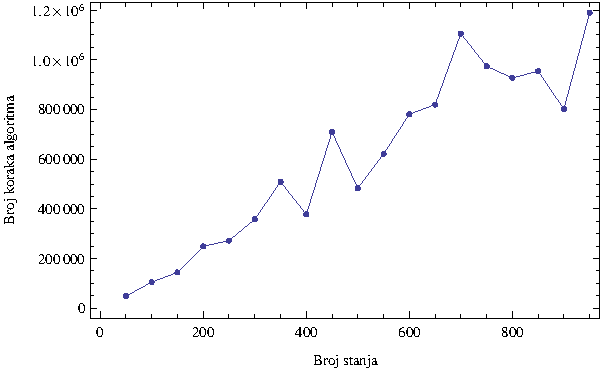
\includegraphics[scale=0.8]{slike/bench1.pdf}
\caption{Broj koraka algoritma u odnosu na broj stanja}
\label{fig:3}
\end{figure}

\begin{figure}[h!]
\centering
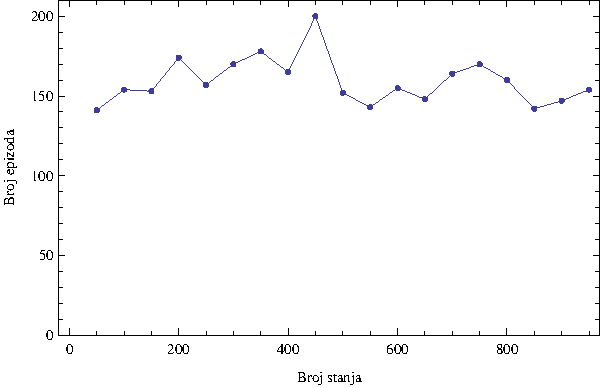
\includegraphics[scale=0.8]{slike/bench2.pdf}
\caption{Broj epizoda u odnosu na broj stanja}
\label{fig:4}
\end{figure}

Slika \ref{fig:4} nam pokazuje broj epizoda u odnosu na broj stanja. Vrijednost matrice $Q$ na ciljnom elementu konvergira
u $100/(1-\gamma)$. Pa kako se $\gamma$ približava 1, ta vrijednost raste i samim tim je potrebno više epizoda da se dostigne.

Slika \ref{fig:5} pokazuje broj epizoda u odnosu na vrijednost $\gamma$. Ako je vrijednost parametra $\gamma$ bliža $0$ agent više preferira veliku nagradu odmah nakon izbora svake akcije, a ako je bliža $1$, agent je spreman pričekati da bi kasnije dobio veću nagradu. Kad bi $\gamma$ bila jednaka $1$, matrica $Q$ ne bi konvergirala.

\begin{figure}[h!]
\centering
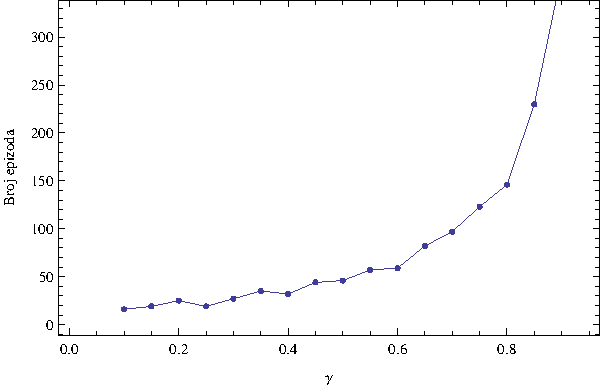
\includegraphics[scale=0.8]{slike/bench3.pdf}
\caption{Broj epizoda u odnosu na vrijednost $\gamma$}
\label{fig:5}
\end{figure}

\section*{Izvori}
\begin{itemize}
\item \emph{Q-Learning By Examples}, Kardi Teknomo, 
\texttt{\small people.revoledu.com/kardi/tutorial/ReinforcementLearning}
\item \emph{Q-learning}, Wikipedia, \\
\texttt{\small en.wikipedia.org/wiki/Q-learning}
\item \emph{Reinforcement Learning Toolbox},\\ 
\texttt{\small www.igi.tugraz.at/ril-toolbox/downloads/index.html}
\end{itemize}
\end{document} 